\chapter{Конструкторская часть}
\hspace{\parindent}В этом разделе будут представлены схемы агоритма линейной обработки данных и конвейерной обработки данных.

\section{Разработка алгоритмов}
\hspace{\parindent}На рис. \ref{fig:linear}-\ref{fig:q3} представлены схемы алгоритма линейной обработки данных, алгоритма конвейерной обработки данных и алгоритмов обрабатывающих устройств.

\begin{figure}[h]
	\centering
    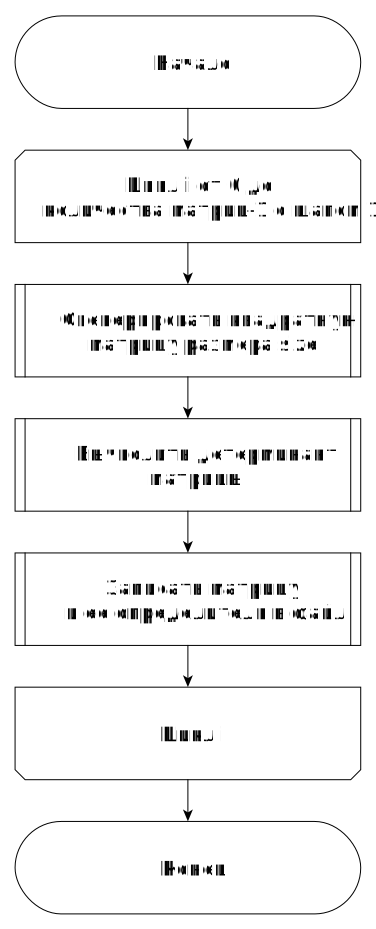
\includegraphics[height=0.8\textheight]{img/linear.png}
    \caption{Алгоритм линейной обработки данных}
    \label{fig:linear}
\end{figure}
\clearpage
\begin{figure}[h]
	\centering
	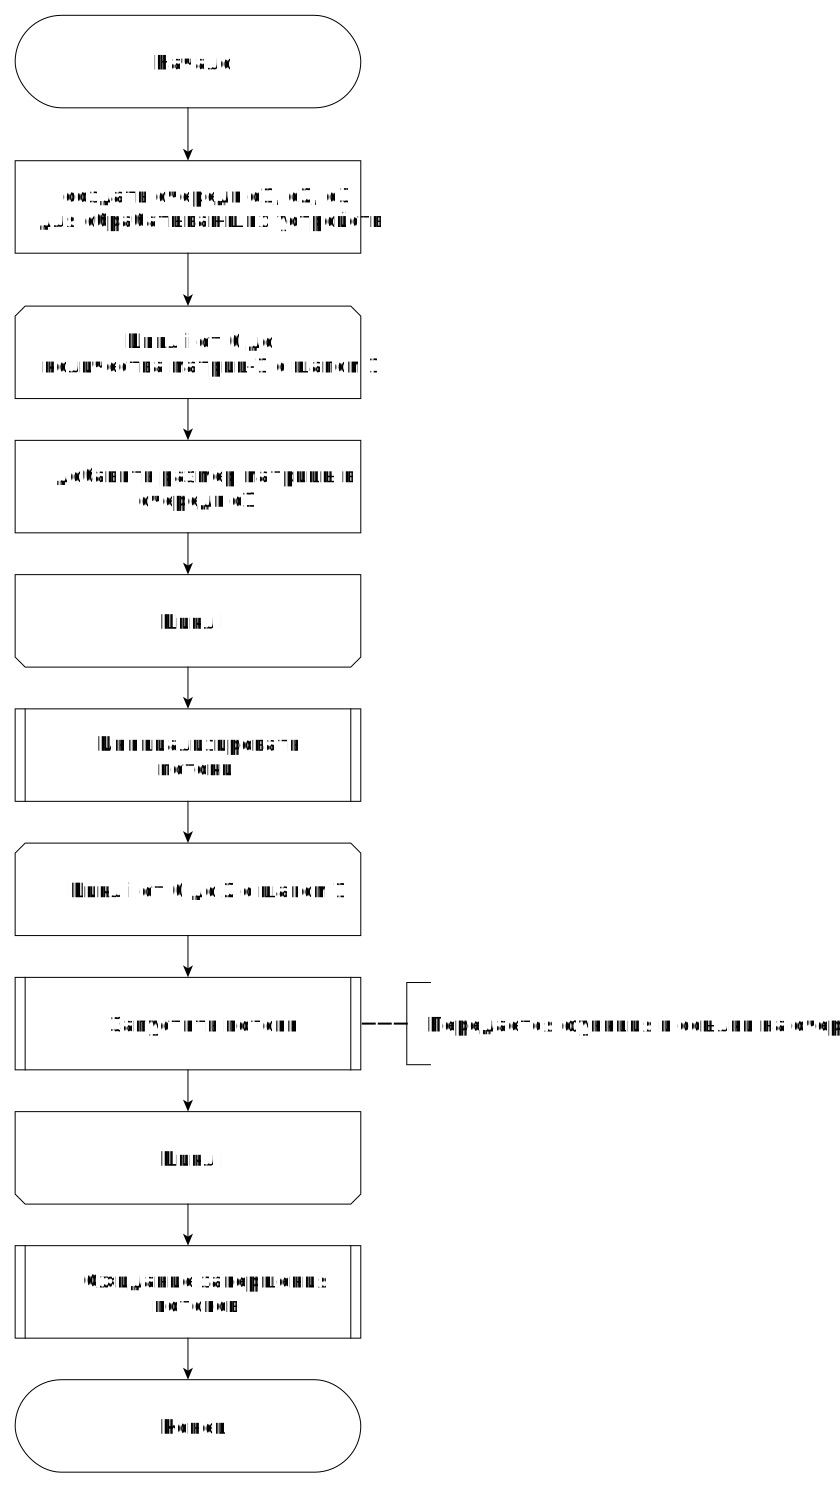
\includegraphics[height=0.8\textheight]{img/conveyor.png}
	\caption{Алгоритм конвейерной обработки данных}
    \label{fig:conveyor}
\end{figure}
\begin{figure}[h]
	\centering
	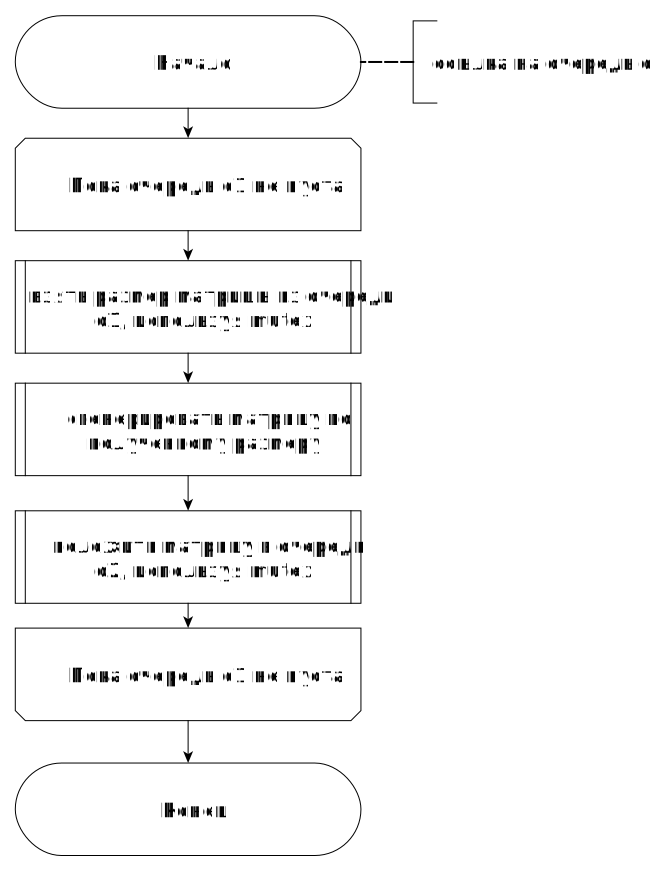
\includegraphics[height=0.5\textheight]{img/q1.png}
	\caption{Алгоритм первого обрабатывающего устройства}
	\label{fig:q1}
\end{figure}
\begin{figure}[h]
	\centering
	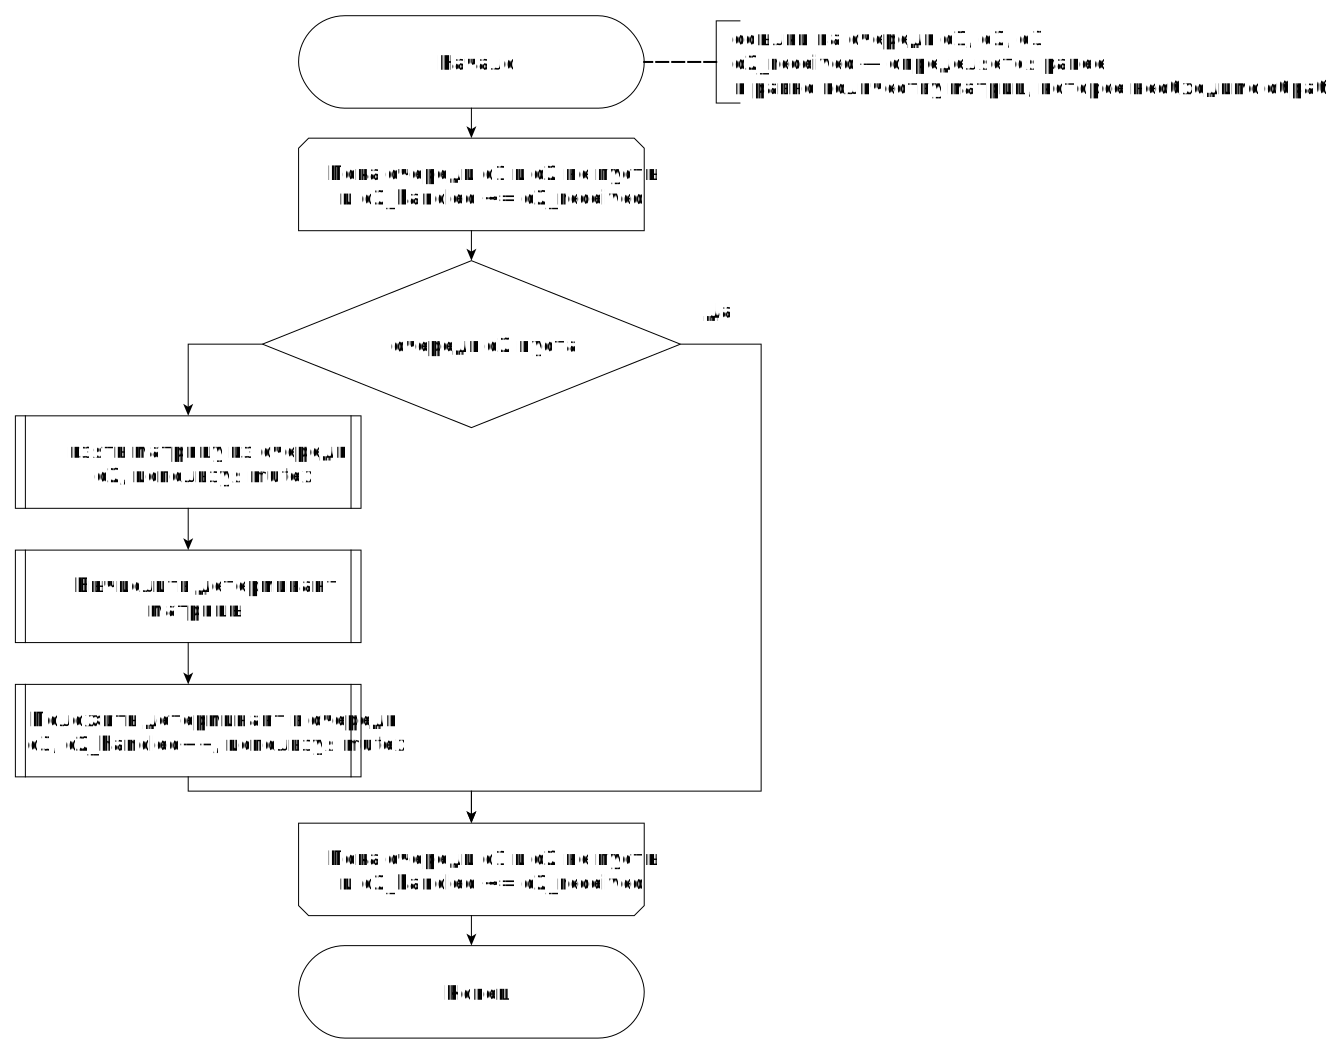
\includegraphics[height=0.5\textheight]{img/q2.png}
	\caption{Алгоритм второго обрабатывающего устройства}
	\label{fig:q2}
\end{figure}
\begin{figure}[h]
	\centering
	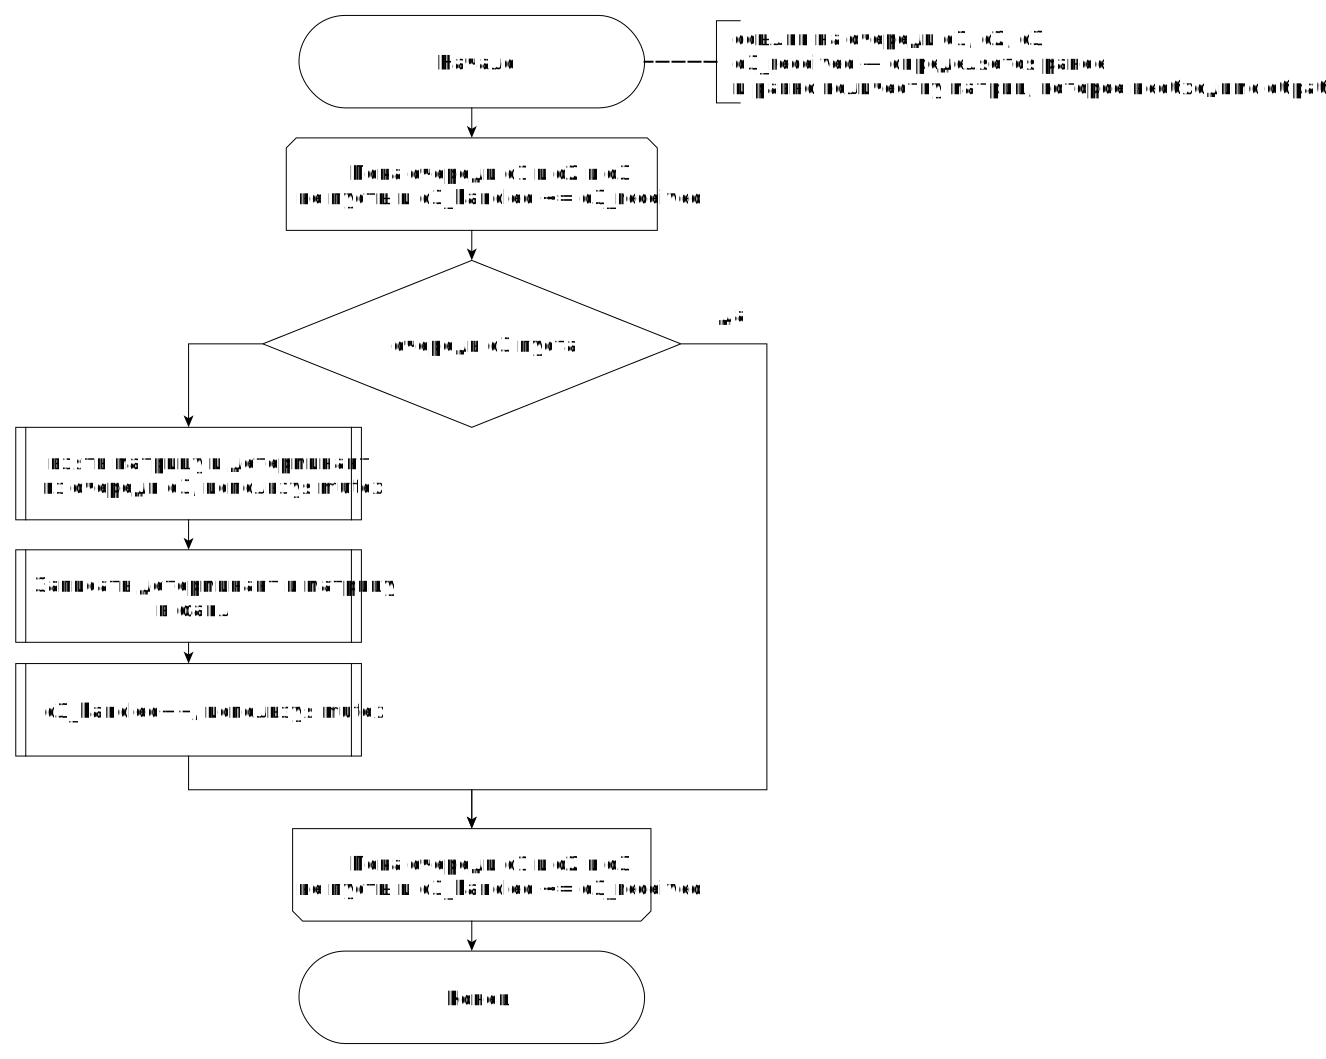
\includegraphics[height=0.5\textheight]{img/q3.png}
	\caption{Алгоритм третьего обрабатывающего устройства}
	\label{fig:q3}
\end{figure}


